%%%%%%%%%%%%%%%%%%%%%%%%%%%%%%%%%%%%%%%%%%%%%%%%%%%%%%%%%%%%%%%%%
% Dissertacao de Mestrado / Dept Fisica, CFM, UFSC              %
% Andre@UFSC - 2011                                             %
%%%%%%%%%%%%%%%%%%%%%%%%%%%%%%%%%%%%%%%%%%%%%%%%%%%%%%%%%%%%%%%%%

%:::::::::::::::::::::::::::::::::::::::::::::::::::::::::::::::%
%                                                               %
%                          Capítulo 2                           %
%                                                               %
%:::::::::::::::::::::::::::::::::::::::::::::::::::::::::::::::%

%***************************************************************%
%                                                               %
%                            Galex                              %
%                                                               %
%***************************************************************%

\chapter{\galex}
\label{sec:Galex}


%***************************************************************%
%                                                               %
%                     Galex - Objetivos                         %
%                                                               %
%***************************************************************%

\section{Objetivos}
\label{sec:Galex:Objetivos}

O {\em Galaxy Evolution Explorer} (\galex) é um telescópio espacial de pequeno
porte da NASA\footnote{{\em NASA Small Explorer} ({\em SMEX}) -
\url{http://explorers.gsfc.nasa.gov/missions.html}}, lançado em 28 de abril de
2003 para conduzir um {\em survey} de todo o céu numa faixa espectral do
ultravioleta (1350--2750\AA). O objetivo principal do \galex{} é estudar a
evolução da taxa de formação estelar em galáxias \citep{Martin2005}. Os dados
coletados pela missão são publicados em {\em Data Releases} periódicos,
denominados {\em General Releases}. Este trabalho foi realizado sobre os dados
do sexto {\em General Release}, GR6.

A missão consiste em uma série de {\em surveys} fotométricos e espectroscópicos
(ver tabela \ref{tab:GalexSurveys}). Destes, os principais {\em surveys} são o
All Sky Survey (AIS) e o Medium Imaging Survey (MIS), que foram utilizados neste
trabalho. O imageamento é feito em duas bandas espectrais: ultravioleta distante
({\em far ultraviolet}, FUV), de 1350 a 1750\AA, e ultravioleta próximo ({\em
near ultraviolet}, NUV), de 1750 a 2750\AA. A curva de transmissão dos filtros
utilizados nessas bandas pode ser visto na figura \ref{fig:GalexFilters}. A
espectroscopia é feita inserindo-se no caminho ótico um {\em grism}, que
consiste num prisma combinado com uma rede de difração. Obtém-se deste modo um
espectro de baixa resolução para cada objeto na imagem, conforme descrito por
\cite{Morrissey2007}.

\begin{table}
	\caption[{\em Surveys} realizados pelo \galex.]{{\em Surveys} realizados pelo
	\galex. O CAI consiste em observações de anãs brancas para calibração. No caso
	do NGS, a magnitude limite é dada em unidades de densidade superficial de
	magnitude. Informações retiradas de \cite{Martin2005}.}
	\begin{tabular}{l r r}
		{\em Survey} & Cobertura do céu ($graus^2$) & Magnitude AB limite \\ 
		\midrule
		{\em Calibration Imaging (CAI)} & - & - \\
		{\em All-sky Imaging Survey (AIS)} & 26000 & 20.5 \\
		{\em Medium Imaging Survey (MIS)} & 1000 & 23 \\
		{\em Deep Imaging Survey (DIS)} & 80 & 25 \\
		{\em Nearby Galaxy Survey (NGS)} & 80 & 27.5 $arcsec^{-2}$  \\
		{\em Wide Field Spectroscopic Survey (WSS)} & 80 & 20 \\
		{\em Medium-deep Spectroscopic Survey (MSS)} & 8 & 21.5--23 \\
		{\em Deep Spectroscopic Survey (DSS)} & 2 & 23--24 \\
	\end{tabular}
	\label{tab:GalexSurveys}
\end{table}

% FIXME: Adicionar figura.
\begin{figure}
	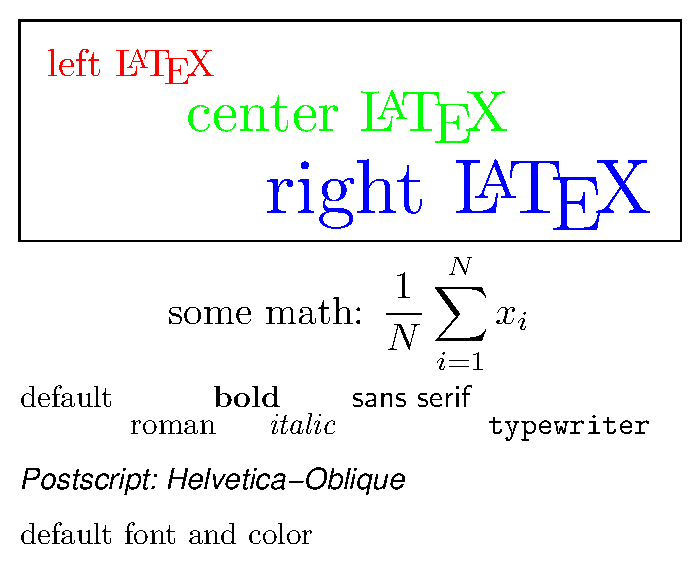
\includegraphics[width=0.5\textwidth]{figuras/test.eps}
	\caption[Curvas de transmissão dos filtros do \galex.]
	{Curvas de transmissão dos filtros do \galex, medidas em
	laboratório \citep{Morrissey2005}.}
	\label{fig:GalexFilters}
\end{figure}



Os {\em surveys} do \galex{} foram planejados de forma a se valer de outros {\em
surveys} já existentes em outros comprimentos de onda. A figura
\ref{fig:GalexSDSSOverlap} mostra a sobreposição da área observada
\footnote{{\em Footprint}, no linguajar astronômico.} pelos surveys AIS e MIS do
\galex{} e do {\em Sloan Digital Sky Survey} (\SDSS). Os objetivos primários da
missão do \galex{} são a calibração da taxa de formação estelar no universo
local, e então determinar o histórico cosmológico de formação estelar entre os
redshifts $0 < z < 2$ \citep{Martin2005}. A comparação com dados de surveys em
outros comprimentos de onda tem um papel fundamental no cumprimento deste
objetivo.

% FIXME: Adicionar figura.
\begin{figure}
	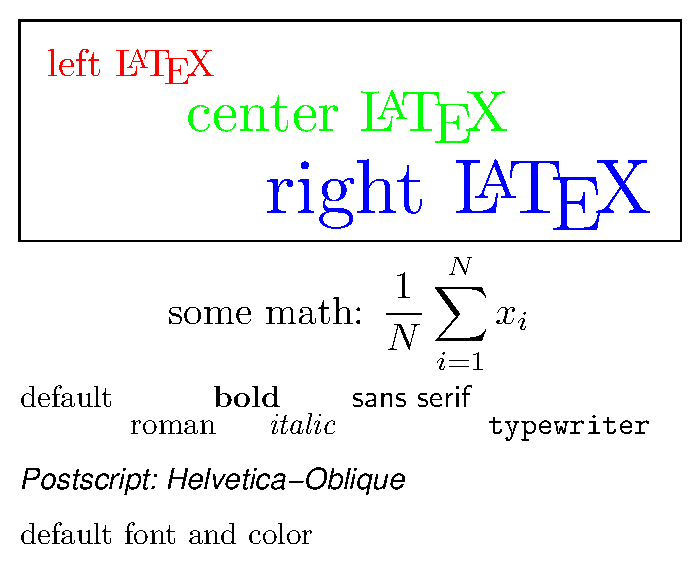
\includegraphics[width=0.5\textwidth]{figuras/test.eps}
	\caption[Footprint dos surveys \galex AIS, MIS e SDSS]
	{Footprint dos surveys \galex AIS, MIS (GR2+3) e SDSS (DR6),
	conforme \cite{Budavari2009}}
	\label{fig:GalexSDSSOverlap}
\end{figure}



%***************************************************************%
%                                                               %
%                Galex - O céu no ultravioleta                  %
%                                                               %
%***************************************************************%

\section{Histórico do estudo do céu no ultravioleta}
\label{sec:Galex:CeuUV}

% FIXME: Usar referência de livro-texto para céu UV.
A camada de ozônio, tão desejável pela proteção que oferece aos seres vivos,
cobra a sua taxa na astronomia. Observações na banda ultravioleta precisam ser
feitas fora da atmosfera terreste, portanto não é de se estranhar que o trabalho
nesta faixa espectral tenha progredido menos do que na faixa do óptico e do
infravermelho.\citneed

% FIXME: adicionar referências.
O primeiro trabalho sistemático de observação UV foi feito pelo {\em Orbiting
Astronomical Observatory 2} \citep{Code1970}, obtendo fotometria e
espectroscopia de estrelas brilhantes, aglomerados globulares e galáxias
próximas. Durante as décadas de 1970 e 1980, este e outros satélites como o TD-1
\citep{Boksenberg1973}, o {\em Astronomical Netherlands Satellite}
\citep{vanDuinen1975} e o {\em International Ultraviolet Explorer}
\citep{Kondo1987} -- o primeiro satélite a utilizar um detetor de imageamento
UV, forneceram os dados fundamentais para os modelos de síntese de população
estelar de galáxias. {\em Surveys} de campo amplo foram feitos por uma camera
lunar erguida por astronautas da {\em Apollo 16} \citep{Carruthers1973}, a bordo
do {\em Skylab} \citep{Henize1975} e pelo instrumento {\em FAUST} a bordo do
{\em Spacelab} \citep{Bowyer1993}. Muitas imagens UV também foram obtidas pelo
{\em Ultraviolet Imaging Telescope} em duas missões em ônibus espacial
\citep{Stecher1997}.

% FIXME: O que é rest-UV?
\cite{Madau1998}
The balloon-borne FOCA Telescope (Milliard et al. 1992) obtained the
first far- UV (FUV) luminosity function for galaxies in the local universe
(Treyer et al. 1998) and the first rest-UV anchor point for the star formation
history plot.


%***************************************************************%
%                                                               %
%                     Galex - Resultados obtidos                %
%                                                               %
%***************************************************************%

\section{Resultados obtidos}
\label{sec:Galex:Resultados}

% FIXME: elaborar sobre as publicações.
o \galex fez o primeiro {\em survey} do céu inteiro em UV. 
\footnote{Lista de publicações do \galex:
\url{http://www.galex.caltech.edu/researcher/publications.html}}



% TODO: resumo de CMD - artigo 1
\cite{Wyder2007} analisa a distribuição de galáxias em função da cor UV e da
magnitude absoluta no universo local. Esta distribuição é conhecida como {\em
Diagrama Cor--Magnitude} (CMD, na sigla em inglês para {\em Color-Magnitude
Diagram}). O autor usa {\em redshifts} e fotometria óptica obtidas do \SDSS
junto com fotometria UV do {\em survey} MIS do \galex. A amostra do \SDSS é
correlacionada com a do \galex{} procurando o objeto do \galex mais próximo de
cada objeto \SDSS até um limite de 4'' (4 segundos de arco).

O diagrama cor-magnitude elaborado por \cite{Wyder2007} mostra a separação das
galáxias nas sequências vermelha e azul (figura \ref{fig:WyderCMD}). Esta
distribuição bimodal é um resultado bem conhecido na astronomia. Porém,
diferente do diagrama cor-magnitude para a faixa espectral do óptico, a
distribuição de cores em UV não pode ser ajustada somente pela soma de duas
gaussianas, há um excesso de objetos nas cores intermediárias entre os picos
vermelho e azul. O autor atribui a boa separação entre as sequências a uma maior
sensibilidade a formação estelar recente.

distribuição bimodal 


We have determined the volume density of galaxies
in the local universe as a function of absolute magnitude Mr;0:1 and ( NUV -
r)0:1 and ( FUV - r)0:1 colors based on a sample of gal- axies observed in the
UV by GALEX and with optical data from the SDSS. The galaxies in these CMDs
separate into well-defined blue and red sequences that become redder with
increasing lu- minosity. While the most luminous galaxies are on the red se-
quence, a separate blue peak is detectable as bright as Mr;0:1 ~= -23. In
contrast to CMDs relying solely on an optical color such as (u - r) (Baldry et
al. 2004), the color distribution at fixed ab- solute magnitude is not well fit
by the sum of two Gaussians due to an excess of objects at intermediate colors
between the blue and red peaks. The greater separation between the blue and red
sequences is a consequence of the greater sensitivity of the UV 314 WYDER ET AL.
bands to very low levels of recent star formation. 

The r0:1-band luminosity
function shape varies systematically with color, with the faint-end slope a
gradually increasing across the blue se- quence, reaching a value of a ~ -0,6
at intermediate colors before increasing even more for the reddest galaxies. We
have used these fits to the luminosity functions to derive the fraction of the
luminosity density in the local universe as a function of color. Dust-free
starburst galaxies with colors ( NUV - r)0,1 < 1 are rare in the local universe
and account for only about 5% of the NUV0:1 luminosity density. About 80% of the
NUV0,1 lumi- nosity density is emitted by blue sequence galaxies with colors
1<(NUV-r)0:1 <3. We have used both the Balmer decrement and the dust-SFH- color
relation of Johnson et al. (2006) to estimate the effect of dust on the galaxy
colors and absolute magnitudes. For the Balmer decrement method, the increase in
color with luminosity along the blue sequence is due entirely to dust with the
dispersion at fixed absolute magnitude relatively unchanged. On the other hand,
the blue sequence color in the CMD corrected for dust using the Johnson et al.
(2006) method does still increase with luminosity, indicating that part of this
change in color is due to the star formation history and not to dust alone. We
argue that we prefer the Johnson et al. (2006) method as it is ultimately based
on an attenuation derived from the FIR / UV ratio. Regardless of which dust
correction we employ, however, a significant number of galaxies remain at colors
in between the two sequences, in- dicating that not all of the galaxies there
are simply dusty ver- sions of blue sequence star-forming galaxies. We have used
the NUV0:1 luminosities corrected for dust using the Johnson et al. (2006)
method in conjunction with the stellar masses determined by Kauffmann et al.
(2003a) to plot the density of galaxies as a function of specific star formation
rate SFR /M* and stellar mass M*. The dispersion in SFR /M* is onlya
factor of 2–3 at a fixed stellar mass along the blue sequence. The value of SFR
/M* decreases from values of ~=10e-9.3 yre-1 at M* ~= 10e8.5 Msun to
~= 10e-10.3 near the tip of the blue sequence at M* = Me11 Msun.
Similar to previous optical results ( Kauffmann et al. 2003a, 2003b), galaxies with low
specific star formation rates begin to dominate above a stellar mass of about
10e10.5 Msun. In addition to the small number of galaxy properties explored
here, many galaxies in our sample contain many other measure- ments mainly from the
SDSS.

In a companion paper in this vol- ume, Martin et al. (2007) have estimated
the mass flux of galaxies from the blue to the red sequence and have discussed
some of the other properties of the galaxies in between the red and blue
sequences.

In another paper, Schiminovich et al. (2007) have inves- tigated the
correlation of morphology and other characteristics with position in the CMD.
While detecting red sequence galaxies out to significant distances in the
rest-frame UV is very difficult, it should be possible to use data from GALEX
deep exposures in conjunction with ground-based photometry and spectra to inves-
tigate the evolution of the blue sequence with redshift. In addi- tion, the
variation of the CMD with local galaxy density should provide interesting
constraints on the nature of the galaxies in between the blue and red peaks as
well as models of the physical processes affecting the evolution of galaxies in
the CMD.


% TODO: CMD - artigo 2
\cite{Schiminovich2007}
We have generated a catalog of galaxies in the local (z < 0:25) universe with a
combination of UV-optical photometry, spec- troscopic measures, structural
parameters, and value-added and physical quantities, and have used it for an
investigation into the distribution of star formation across galaxies of
different mor- phologies and stellar masses. Our chief results are as follows.
1. We have derived a new set of physical properties of the galaxies in our
samples, including star formation and stellar mass rates and surface densities,
dust attenuations, and gas fractions. Our measurements incorporate a slightly
modified prescription for dust attenuation, designed to use the best available
data to derive star formation rates across the whole galaxy sample. In general,
this follows most closely the approaches described in Johnson Fig. 26.—Estimated
stellar mass flux density off of the SF sequence and comparison with the SFR
density vs. M? . Solid lines: Total stellar mass flux density for all galaxies
(black) and bulge-dominated galaxies (red ) with log sum SFR > 0:5. Green dotted
line: Stellar mass flux rate for transition galaxies from Paper III (Table 3).
Dashed lines: SFR density vs. M? for total (black), disk-dominated (blue), and
bulge-dominated (red ) subsamples. Values are per 0.3 dex M? bin. et al. (2007)
and Kauffmann et al. (2003a), but ultimately we hope to develop it as a
refinement over current methodology. 2. For the first time, we have measured the
local UV lumi- nosity function against galaxy structural parameters as well as
inclination. Among our key results is that we have shown that the fraction of
intermediate and early-type galaxies is highest for the most UV luminous
galaxies, dropping off to low frac- tions for the least luminous galaxies. 3.
Throughout this study, our emphasis has been on the prop- erties of galaxies on
and off of a local ‘‘star-forming sequence’’ defined by log SFR /M* SUM
0:36 log M 6:4. We find, among other trends, that our measure of the star
formation rate surface density, Sum SFR (measured within ru;50) is nearly
constant along this sequence. 4. We have split our sample into disk and bulge-dominated
galaxies using the i-band Sersic index, and find that disk gal- axies occupy a
very tight locus in SFR vs. M? space, while bulge- dominated galaxies display a
much larger spread of SFRs at fixed stellar mass. In particular, a significant
fraction of galaxies with SFR and sumSFR above those on the ‘‘star-forming
sequence’’ are bulge-dominated. 5. We have used our derived distribution
functions to ask whether a significant fraction of these galaxies may be
experienc- ing a final episode of star formation ( possibly induced by merger of
other bursts), soon to be quenched, by determining whether this population can
explain the growth rate of the non-star-forming population We find that this is
a plausible scenario for bulge- dominated galaxies near the characteristic
transition mass under reasonable assumptions regarding quenching timescales. We
use this technique to estimate the rate of mergers/starbursts that take galaxies
off of the star-forming sequence and show that the im- plied merger rates are
consistent with local measurements.


% TODO: CMD - artigo 3
\cite{Martin2007}
We have introduced a new quantity, the mass flux density of galaxies evolving
from the blue sequence to the red sequence. We developed a simple technique for
constraining this mass flux that exploits the excellent separation of red and
blue sequences in the NUV - r band Hess function. We used the volume-corrected
number density in the extinction-corrected UV-optical color- magnitude
distribution, the stellar age indexes HdeltaA and Dn (4000), and a simple
prescription for spectral evolution using a quenched
starformationhistory. Our estimated mass flux M yr1 Mpc3,
although strictly an upper limit, compares favorably with estimates of the
average mass flux that we make based on the optical and UV data. Galaxies in the
transition zone are pref- erentially AGNs, although we find at best weak
evidence that the quench rates are higher in higher luminosity AGNs. We note
that our technique could be applied with alternative evolutionary clocks, such
as morphology. Our approach using a single color and spectral index was simple,
but a more refined tech- nique would use the entire spectral energy distribution
in addi- tion to any relevant spectral indices. Our simple approach is fairly
easy to apply to deep galaxy surveys, future work will study the evolution of
the mass flux as well as its dependence on galaxy density and environment. Falar
da bimodalidade. Conclusões dos principais artigos.


% FIXME: Adicionar figura - diagrama cor-magnitude.
\begin{figure}
	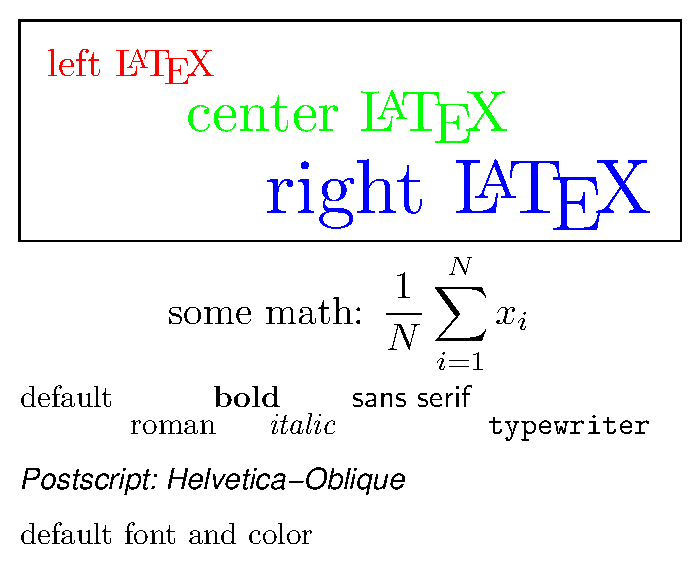
\includegraphics[width=0.5\textwidth]{figuras/test.eps}
	\caption[Diagrama cor-margnitude em ultravioleta.]
	{Diagrama cor-margnitude em ultravioleta. Figura 7 de \cite{Wyder2007}.}
	\label{fig:WyderCMD}
\end{figure}



%***************************************************************%
%                                                               %
%                     Galex - Banco de dados                    %
%                                                               %
%***************************************************************%

\section{Data releases e banco de dados}
\label{sec:Galex:BancoDeDados}

% FIXME: Arrumar uma tradução melhor para ``tile''.
Os dados obtidos pelo \galex{} são armazenados no {\em Multi-Mission archive at
the Space Telescope Science Institute} (MAST). O acesso a estes dados é público,
a liberação é feita anualmente em {\em General Releases} (GR). Os dados
consistem basicamente em imagens e catálogos, dividos em campos ({\em tiles})
com área de aproximadamente 1,2 graus quadrados. Devido ao modo como o \galex{}
faz as observações, um determinado objeto pode estar presente em mais de um campo. A
tabela \ref{tab:GalexReleases} mostra o número cumulativo de campos observados
por {\em survey} em cada GR\footnote{Informações retiradas do website do GR6:
\url{http://galex.stsci.edu/GR6/}}. Observações de pesquisadores convidados
({\em Guest Investigators}, GI) foram selecionadas de forma a complementar os
{\em surveys}.

\begin{table}
	\caption[Campos observados em cada {\em General Release} do \galex.]{Campos
	observados em cada {\em General Release} do \galex.}
	\begin{tabular}{l r r r r r r r r}
		{\em Release} & AIS   & DIS & MIS  & NGS & GI   & CAI & Espectros & Total \\
		\midrule
		GR1           & 3074  & 14  & 112  & 52  & -    & -   & 7         & 3259  \\
		GR2/GR3       & 15721 & 165 & 1017 & 296 & 288  & 20  & 41        & 17548 \\
		GR4/GR5       & 28269 & 292 & 2161 & 458 & 788  & 38  & 174       & 32180 \\
		GR6           & 28889 & 338 & 3479 & 480 & 1314 & 51  & -         & 34551 \\
	\end{tabular}
	\label{tab:GalexReleases}
\end{table}

Para facilitar o acesso aos dados do \galex, o MAST desenvolveu uma ferramenta
chamada {\em GalexView}, utilizando tecnologia {\em Adobe Flex}\footnote{{\em
Adobe Flex} é um {\em framework} de código aberto que permite desenvolver
aplicações para {\em web browsers}. Ver
\url{http://www.adobe.com/products/flex.html}.}. Desta forma o {\em GalexView }
pode ser acessado através de seu {\em website}\footnote{GalexView:
\url{http://galex.stsci.edu/GalexView/}} em qualquer {\em web browser} que tenha
suporte ao {\em Adobe Flash Player}\footnote{{\em Adobe Flash Player} é uma
extensão multiplataforma para {\em web browsers} que provê capacidade de
visualização de conteúdo {\em flash} gerado tanto pelos seus editores
proprietários quanto por ferramentas de terceiros. Ver
\url{http://www.adobe.com/products/flashplayer/}.}.

Através do {\em GalexView} é possível fazer buscas, visualizar e obter imagens e
catálogos dos campos do \galex. As buscas podem ser feitas de forma bastante
versátil, tanto pelo nome do objeto quanto pelas coordenadas do céu. O formato
de entrada é flexível o suficiente para evitar os problemas causados por
idiosincrasias na notação de coordenadas (por exemplo, tanto ``14h03m12.6s
+54d20m56.7s'' quanto ``14 03 12.6 54 20 56.7'' ou ``210.83 54.35'' apontam para
a mesma região). A sua interface (figura \ref{fig:GalexView}) permite filtrar o
conteúdo retornado pelas buscas, separando por {\em surveys}. Há também uma
ferramenta de histograma, permitindo filtrar pelos valores das colunas dos
catálogos. Os objetos selecionados na busca aparecem marcados na visualização da
imagem. Utilizando um sistema do tipo ``carrinho de compras'', pode-se
selecionar campos e objetos de interesse, para ao final do uso do sistema baixar
toda a seleção de uma vez.

% FIXME: Adicionar figura.
\begin{figure}
	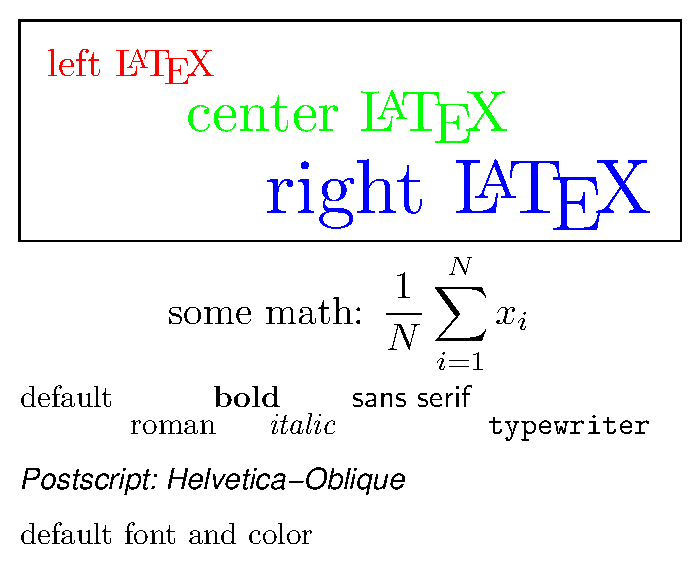
\includegraphics[width=0.5\textwidth]{figuras/test.eps}
	\caption[Tela do programa GalexView.]
	{Tela do programa GalexView.}
	\label{fig:GalexView}
\end{figure}

Tanto o {\em GalexView} quanto outras ferramentas de busca do MAST, como o
\galex {\em Search Form} e o \galex {\em Tilelist}, são construídos sobre um
{\em banco de dados relacional} acessado através da linguagem {\em SQL}
\citep{Chamberlin1974}. Muito comum na indústria, bancos de dados relacionais
dispõem em geral uma vasta gama de ferramentas para gerenciamento dos dados. Uma
de suas grandes vantagens é o uso de {\em índices} para agilizar o acesso a
dados. Embora a tecnologia exista desde a década de 1970 \citep{Codd1970}, até
uma década atrás suas vantagens eram praticamente neglicenciadas na astronomia.

Tradicionalmente astrônomos armazenam seus dados em arquivos texto ou binários
contendo um registro por linha, de um forma tecnicamente conhecida como {\em
flat file}. Buscas neste tipo de banco de dados são feitas examinando
individualmente cada registro do arquivo. Com o volume de dados obtido pelo
\galex (aproximadamente 222 milhões de objetos, 34 mil campos)\citneed, o uso
de arquivos simples para armazenamento de dados se torna inviável.\citneed É
preciso ``profissionalizar'' o gerenciamento de dados de um {\em survey} desta
escala.

Bancos de dados relacionais e ferramentas para gerenciamento e acesso a dados
serão tratados com mais detalhes no capítulo \ref{sec:Crossmatch}.



% End of this chapter
